
\documentclass[12pt,epsfig,color,russian]{article}
\usepackage[russian]{babel}
\usepackage{epsfig}
\usepackage{color}

\topmargin=0cm
\hoffset -30mm
\voffset -12mm
\setlength{\unitlength}{1mm}
\parindent=10mm
\textheight=250mm
\textwidth=190mm
\pagestyle{empty}

\begin{document}
\vspace*{-20mm}
 \centerline{\underline{\huge\bf Классическая электронная теория}}\vspace{5mm}
 Ток в металлах не меняет их химических свойств $\Rightarrow$ это движение не атомов, а только электронов ($e^-$). Приходится допустить, что там $\exists$ (частичная?) диссоциация на +ионы и $e^-$, которые хаотично движутся с какой-то средне-квадратичной скоростью $\overline{u}$ (распределение Максвелла). Приложенное поле $\vec{E}$ увлекает их в определенном направлении $\Rightarrow$ появляется эл. ток $I$.\\
 \begin{picture}(190,35)(0,0)
 \put(10,0){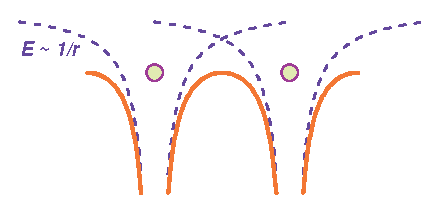
\includegraphics{GP017F01.eps}}
 \put(90,0){\includegraphics{GP017F02.eps}}
 \end{picture}\\
 $\forall$ +иона $\exists$ поле $E_{\rm pot}\sim1/r$. Эти поля от соседних ионов складываются, и в металле получается периодический набор "ям", по которым "гуляют" свободные $e^-$. Снаружи потенциал > чем внутри:
 $\overline{E_a}<E_0$. Если положить, что снаружи $E_0=0$, то внутри -- яма $E_a<0$. У свободного $e^-$ энергия
 $E_a<E<E_0$  $\Rightarrow$ он свободен внутри, но не может выйти наружу.

 \underline{Эксперимент:} если проводник разогнать, а потом тормознуть, то все свободные $e^-$ по инерции дернутся вперед, и появится импульс тока. Оценим масштаб:

 Пусть скорость =$v_0$, тормозим с ускорением =$-a$. Относительно проводника у $e^-$ появляется ускорение $+a$, как если бы на них действовало поле $E$:
 \begin{displaymath}
 E=\frac{f}{e}=\frac{ma}{e}.
 \end{displaymath}
 Если длина проводника =$L$, то на его концах возникнет разность потенциалов
 \begin{displaymath}
 V_1-V_2=E\cdot L=\frac{f}{e}=\frac{m}{e}\cdot a\cdot L
 \end{displaymath}
 и потечет ток
 \begin{displaymath}
 I=\frac{V_1-V_2}{R}=\frac{m}{e}\cdot \frac{a}{R}\cdot L
 \end{displaymath}
Если время полного торможения =$t$, то $a=v_0/t$, и ток =
 \begin{displaymath}
 I=\frac{m}{e}\cdot \frac{v_0}{Rt}\cdot L
 \end{displaymath}
Заряд, протекший через проводник:\vspace{-3mm}
 \begin{displaymath}
 Q=I\cdot t=\frac{m}{e}\cdot \frac{v_0}{R}\cdot L
 \end{displaymath}
Можно экспериментально измерить $\frac{m}{e}$ или  $\frac{e}{m}$ !!!

Мандельштам и Папалекси (СПб, 1913 г.) крутили туда-сюда катушку с длинным проводом и слышали звук в наушнике.\\
Количественное измерение: Стюарт и Толмен (катушка + баллистический гальванометр). Реультат:
\begin{enumerate}
\item свободные заряды ОТРИЦАТЕЛЬНЫ
\item $\frac{e}{m}=4.8\cdot 10^{17}$ CGSE/г
\end{enumerate}
Из опытов Милликена: $e=4.808\cdot10^{-10}$ CGSE и поэтому  $\Rightarrow$ $m_e=9.1\cdot10^{-28}$ г $\simeq\frac1{1838}$ a.m.u.\\[3mm]

{\bf\Large Закон Ома и закон Джоуля-Ленца с этой точки зрения --?}\\[2mm]
Лоренц: $\exists$ как бы "Электронный газ" с плотностью $n_0$ (порядка числа атомов в ед-це объема = $N\cdot\frac{\rho}{\mu}$) $\Rightarrow$ $\exists$ средний пробег $\overline{\lambda}$, среднее время между столкновениями  $\overline{\tau}=\overline{\lambda}/\overline{u}$ и среднее число столкнований в ед-цу времени $\overline{z}=1/\overline{\tau}$.

Должно быть термодинамическое равновесие между атомами и свободными $e^-$, т.е., они имеют одинаковую $T$ и $\Rightarrow$ среднюю кинетическую энергию.  Но для атомов $E_k=\frac32kT$,  $\Rightarrow$ для электронов
 \begin{displaymath}
 \frac{m\overline{u}^2}2 = \frac32kT\hspace{10mm}\Rightarrow\hspace{10mm}\overline{u}=\sqrt{\frac{3kT}{m}}
 \end{displaymath}
Каков масштаб $\overline{u}$?  Масса эл-на меньше массы атома в 1838$\cdot A$ раз, а энергии равны  $\Rightarrow$ скорость больше в $\sqrt{1838\cdot A}\simeq 43\sqrt{A}$ раз. Для атомов это км/с, а для эл-нов -- 100 км/с.

Эта скорость -- хаотична, и тока не дает. При наличии поля на нее накладывается другая, направленная, скорость $\overline{v}$. Тогда поток эл-нов составит $n_0\overline{v}$, а поскольку каждый из них несет заряд $e$, то плотность тока (заряд через ед-цу площади в ед-цу времени)
 \begin{displaymath}
 i=e\,n_0\,\overline{v}
 \end{displaymath}
Каков масштаб $\overline{v}$? Пусть плотность тока = 100 А/см$^2=3\cdot10^{11}$ CGSE/см$^2$. Тогда для меди (A=64 г/моль, $\rho$=8.9 г/см$^3$) получим:
 \begin{displaymath}
 \overline{v}=\frac{i}{n_0e}=\frac{i\cdot\mu}{N\rho e}\simeq\frac{3\cdot10^{11}\cdot64}{6\cdot10^{23}\cdot8.9\cdot4.8\cdot10^{-10}}\sim 10^{-2}
 \end{displaymath}
Размерность -- см/с.  То есть, это 0.1 мм/с! Видим, что это ОЧЕНЬ малая скорость (по сравнению с тепловой).\\[2mm]

Теперь свяжем плотность тока с напряженностью поля. Сила, действующая на электрон: $f=eE$ (на самом деле $-eE$, потому что заряд эл-на -- отрицателен). Ускорение: $a=\frac{f}{m}=\frac{e}{m}E$. После каждого столкновения вся набранная скорость теряется, и все начинается сначала. За каждый пробег набирается скорость $v_0=\tau a=\tau\frac{e}{m}E$, а в среднем она равна половине:
 \begin{displaymath}
 \overline{v}=\frac12v_0=\frac{eE}{2m}\cdot\overline{\tau}=\frac{eE}{2m}\cdot\frac{\overline{\lambda}}{\overline{u}}
 \end{displaymath}
Плотность тока:
 \begin{displaymath}
 i=e\,n_0\,\overline{v}=\frac{e^2n_0\overline{\lambda}}{2m\overline{u}}\cdot E
 \end{displaymath}
Первый множитель постоянен для данного проводника, и если его принять за проводимость, то получим {\bf закон Ома}:
 \begin{displaymath}
 i=\sigma\,E,\hspace{10mm}\texttt{где}\hspace{10mm}\sigma\equiv \frac{e^2n_0\overline{\lambda}}{2m\overline{u}}
 \end{displaymath}
В конце каждого пробега набирается направленная скорость $v_0=\tau a=\tau\frac{e}{m}E=\frac{\overline{\lambda}}{\overline{u}}\cdot\frac{e}{m}E$, а энергия этого направленного движения
 \begin{displaymath}
 E_k =\frac{m\overline{v_0}^2}2    =\frac12\cdot \frac{e^2E^2\overline{\lambda}^2}{m\overline{u}^2}
 \end{displaymath}
Вся она отдается атомам проводника $\overline{z}=1/\overline{\tau}=\overline{u}/\overline{\lambda}$ раз в секунду. Если учесть, что число таких электронов = $n_0$, то для общего энерговыделения в ед-це объема за секунду получим {\bf закон Джоуля-Ленца}:
 \begin{displaymath}
 w=E_k\cdot n_0\cdot\overline{z}  =\frac12\cdot \frac{n_0\,e^2\,E^2\,\overline{\lambda}}{m\overline{u}}=\sigma\,E^2
 \end{displaymath}\\[3mm]

{\bf\Large Связь электро- и теплопроводности в металлах --?}\\[2mm]
Металлы: хорошая электро- и теплопроводность, а диэлектрики -- плохая. Может, хорошая тепло\-про\-вод\-ность металлов тоже обусловлена свободными эл-нами?

Для коэффициента теплопроводности газов мы получали:
 \begin{displaymath}
\chi =\frac13\,n_0\,\overline{\lambda}\,\overline{u}\,\frac{i}2k
 \end{displaymath}
полагая число степеней свободы $i=3$, получим для теплопроводности "электронного газа":
 \begin{displaymath}
\chi =\frac12\,n_0\,k\,\overline{\lambda}\,\overline{u}
 \end{displaymath}
Тогда, если тепло- и электро-проводности пропорциональны друг другу, то, наверное, их отношение должно быть какой-то константой?...
 \begin{displaymath}
\frac{\chi}{\sigma} =\frac{\frac12\,n_0\,k\,\overline{\lambda}\,\overline{u}}{\frac{e^2n_0\overline{\lambda}}{2m\overline{u}}}=
\frac{m\,\overline{u}^2}{e^2}k
 \end{displaymath}
 Но $mu^2/2$ -- это энергия, которая должна соответствовать данной температуре металла:
 \begin{displaymath}
\frac{m\,\overline{u}^2}2=\frac32kT\hspace{10mm}\Rightarrow\hspace{10mm}
\frac{\chi}{\sigma}\;=\; \frac{3k^2}{e^2}T \simeq 5.3\cdot10^{-9}\cdot T
 \end{displaymath}
(если измерять все в Омах, см, градусах, секундах и калориях). Получился {\bf закон Видемана-Франца}, экспериментально обнаруженный ими в 1853 году. Они получили очень похожее число (от 4.6 до 5.6 для разных металлов).

В действительности все не так.  Электропроводность зависит от  $T$ через скорость теплового движения эл-нов $\overline{u}$:
 \begin{displaymath}
\sigma= \frac{e^2n_0\overline{\lambda}}{2m\overline{u}}
 \end{displaymath}
 Мы (как и Лоренц) считали, что $\overline{u}\sim \sqrt{T}$, и тогда должно быть $\sigma\sim1/\sqrt{T}$. Но ведь из электротехники хорошо известно, что $\rho\sim T$, и $\Rightarrow$ $\sigma\sim1/T$.

Другое противоречие -- в том, что раз эл-ны двигаются и имеют $E_k$, то теплоемкость у металлов должна быть не $\frac{i}{2}R$, а $\frac{i+3}{2}R$, то есть, раза в 1.5--2 больше, чем у изоляторов. Но это не так.  $\Rightarrow$ электроны, участвующие в электро- и теплопроводности, не влияют (почему-то) на теплоемкость.\\[5mm]
 \centerline{\underline{\huge\bf Квантовая теория эл.-проводности металлов}}\vspace{5mm}

Все противоречия снимаются в кватовой механике, где система частиц может иметь лишь дискретный набор возможных состояний (а не их сплошной спектр). Если потенциальная энергия электрона в атоме $E_p=-C/r$, то по квантовой теории электрон может находиться лишь в одном из состояний (уровней): $E_n=-B/n^2$, где $n$ -- целое число ($n=1,2,3..$).

То же самое и в кристалле, но там уровней очень много, и они расположены намного чаще. \\
 \begin{picture}(190,30)(0,0)
 \put(10,0){\includegraphics{GP017F03.eps}}
 \put(100,0){\includegraphics{GP017F04.eps}}
 \end{picture}\\
Казалось бы: какая разница? Но тут в дело вступает принцип Паули, запрещающий находиться двум одинаковым частицам в одном и том же состоянии. Так как у электрона может быть 2 проекции его спина ($\pm1/2$), то на один уровень может поместиться $\leq2$ электронов. Таким образом, распределение N свободных электронов по энергии отличается от больцмановского. Например, при $T=0$ по "классике" все электроны должны лежать на дне ямы, а по "квантам" они заполнят N/2 самых нижних уровней, а остальные будут пусты. При более высокой температуре это распределение будет описываться функцикй Ферми (при очень высокой $T$ она превращается в распределение Больцмана).\\
 \begin{picture}(190,50)(0,0)
 \put(65,0){\includegraphics{GP017F05.eps}}
 \put(0,40){\makebox(0,0)[lt]{\parbox{60mm}{
 Распределение элек\-т\-ро\-нов по уровням (ве\-ро\-ят\-ность того, что уро\-вень с дан\-ной энер\-ги\-ей за\-нят).
 }}}
 \end{picture}\\
Приложенное поле передает электронам некую энергию, переводя их на более высокие (незанятые) уровни и придавая им направленную скорость. Появляется ток. Ненулевое сопротивление объясняется рассеянием волн на неоднородностях кристалла, причем зависимость проводимости от температуры носит как раз нужный характер: $\sigma\sim1/T$.\\

С теплоемкостью тоже все проясняется: при не слишком высоких $T$ большинство электронов сидит на нижних уровнях и их ОБЩАЯ энергия от $T$ почти не зависит. Поэтому и на теплоемкость они не влияют. Действительно, если учесть, что уровни расположены неравномерно (чем выше -- тем чаще), и нарисовать распределение Ферми не по уровням, а по энергии, то увидим, что центр тяжести распределения с ростом $T$ сдвигается очень слабо.\\
 \begin{picture}(190,50)(0,0)
 \put(65,0){\includegraphics{GP017F06.eps}}
 \put(0,40){\makebox(0,0)[lt]{\parbox{60mm}{
 Распределение элек\-т\-ро\-нов по энергии (ве\-ро\-ят\-ность най\-ти элек\-трон в дан\-ном ин\-тер\-ва\-ле энер\-гии).
 }}}
 \end{picture}\\

Объясним контактную разность потенциалов. Для этого рассмотрим два металла A и B. Элек\-тро\-ны в металле А находятся в потенциальной яме, занимая нижние N/2 уровней, вплоть до энергии
\\
 \begin{picture}(190,30)(0,0)
 \put(0,0){\includegraphics{GP017F09.eps}}
 \put(80,29){\makebox(0,0)[lt]{\parbox{110mm}{
 $E_i$ -- энергии Ферми, характерной для данного металла. Чтобы электрон вышел наружу, он должен преодолеть разность потенциалов между $E_i$ и потенциалом вне металла, т.е. $E_0$. Эта разность называется РАБОТОЙ ВЫХОДА; обычно она составляет единицы Вольт.
  }}}
 \end{picture}\\

 \begin{picture}(190,50)(0,0)
 \put(0,0){\includegraphics{GP017F07.eps}}
 \put(90,0){\includegraphics{GP017F08.eps}}
 \end{picture}\\

\end{document}
